%!TEX root = ../thesis.tex
%*******************************************************************************
%****************************** Second Chapter *********************************
%*******************************************************************************
\chapter{Equations, images and algorithms}
This chapter shows you how to write complex equation and position complicated images.
\section{Image with tikz label}
\begin{figure}[htbp!]
\centering
	\begin{tikzpicture}
		    \node[anchor=south west,inner sep=0] (image) at (0,0) {\includegraphics[page = 4, width=0.8\textwidth]{Ch2_Images/MathPreliminariesFigure.pdf}};
	    \begin{scope}[x={(image.south east)},y={(image.north west)}]
	        % \draw[help lines,xstep=.1,ystep=.1] (0,0) grid (1,1);
	        % \foreach \x in {0,1,...,9} { \node [anchor=north] at (\x/10,0) {0.\x}; }
	        % \foreach \y in {0,1,...,9} { \node [anchor=east] at (0,\y/10) {0.\y}; }
	        \node[draw = none, fill = none, color = blue] at (0.52, 0.57) {\Large{$x$}};
	        \node[draw = none, fill = none, color = blue] at (0.38, 0.9) {\Large{$y$}};
	        \node[draw = none, fill = none, color = blue] at (0.93, 0.37) {\Large{$\alpha$}};
	        \node[draw = none, fill = none, color = blue] at (0.775, 0.72) {\Large{$\beta$}};
	        \node[draw = none, fill = none, color = blue] at (0.84, 0.28) {\Large{$z$}};
	        \node[draw = none, fill = none, color = red] at (0.85, 0.43){\Large{$P_0$}};
	        \node[draw = none, fill = none, color = red] at (0.338, 0.39){\Large{$P_1$}};
	        \node[draw = none, fill = none, color = white] at (0.26, 0.3){\Large{$S$}};
	        \node[draw = none, fill = none, color = blue] at (0.55, 0.33){\Large{$r_{01}$}};
	        \node[draw = none, fill = none] at (0.15, 0.15){\Large{Plane waves}};
	    \end{scope}
	\end{tikzpicture}
\caption{The coordinate system for analyzing different diffraction regimes}
\label{Fig:DiffractionViaAperature}
\end{figure}

\subsection{Equation 1}
Consider the geometry shown in Figure. \ref{Fig:DiffractionViaAperature}, coordinates $(x, y)$ and $(\alpha,\beta)$ locates at the aperture plane and the observation plane respectively. Setting $r_{01}$ as the distance between $P_0$ and $P_1$, the Rayleigh-Sommerfeld relationship becomes:
\begin{equation}
	U(\alpha, \beta) = \frac{z}{j\lambda}\iint_\Sigma U(x, y)\frac{\exp{jkr_{01}}}{r_{01}^2}dxdy
	\label{eq:FresnelDiffraction}
\end{equation}
where, $r_{01} = \sqrt{z^2+(\alpha - x)^2+(\beta-y)^2}$. The complexity of $r_{01}$ suggests further assumptions to simplify Equation. \ref{eq:FresnelDiffraction}. Assume $P_0$ and $P_1$ are reasonably coaxial, then $r_{01}$ in the denominator approximates to $z$. However, it is the fact that small perturbation in the exponential function might lead to huge changes. The simplification of the distance term requires other approach. Binomial expansion is therefore adopted on $r_{01}$ to eliminate the square root.
\begin{equation}
	r_{01} \approx z\left\{1+\frac{1}{2}  \left[\left(\frac{\alpha-x}{z}\right)^2+\left(\frac{\beta-y}{z}\right)^2 \right]\right\}
	\label{eq:r01BinomialExpansion}
\end{equation} 
Substitution Equation.\ref{eq:r01BinomialExpansion} into Equation.\ref{eq:FresnelDiffraction} yields the Fresnel diffraction integral:
\begin{equation}
	U(\alpha, \beta) = \frac{e^{jkz}}{j\lambda z}e^{j\frac{k(\alpha^2+\beta^2)}{2z}}\iint\left\{U(x,y)e^{j\frac{k(x^2+y^2)}{2z}}\right\}e^{-j\frac{2\pi}{\lambda z}(\alpha x+\beta y)}dxdy
	\label{eq:FresnelDiffractionIntegralFomula}
\end{equation}
The above equation suggests a significant conclusion: the diffraction pattern is the Fourier transform of a quadratic phase modulated aperture, multiplied with a scaling factor.

\subsection{Cross reference equations and images}
Fraunhofer diffraction deals with light propagation in the far field. In this regime, the quadratic phase term in Equation.\ref{eq:FresnelDiffractionIntegralFomula} can be dropped to make the whole equation even simpler:
\begin{equation}
	U(\alpha, \beta) = \frac{e^{jkz}}{j\lambda z}e^{j\frac{k(\alpha^2+\beta^2)}{2z}}\iint U(x,y)e^{-j\frac{2\pi}{\lambda z}(\alpha x+\beta y)}dxdy
	\label{eq:FraunhoferDiffractionFormula}
\end{equation}
Normalizing above equation, and letting $u = \frac{k\alpha}{2\pi z}$, $v = \frac{k\beta}{2\pi z}$ \cite{4B11}, the final relationship becomes:
\begin{equation}
	U(u,v) = \iint U(x,y)e^{-j2\pi(ux+vy)}dxdy
	\label{FourierTransformOfLight}
\end{equation}
Figure \ref{cubicAperture} and \ref{circularAperture} visualized a plane wave traversing a cubic or a circular aperture respectively.
\section{Two images in the same row}
\begin{figure}[htbp!]
	\begin{subfigure}{0.5\linewidth}
		% \centering
		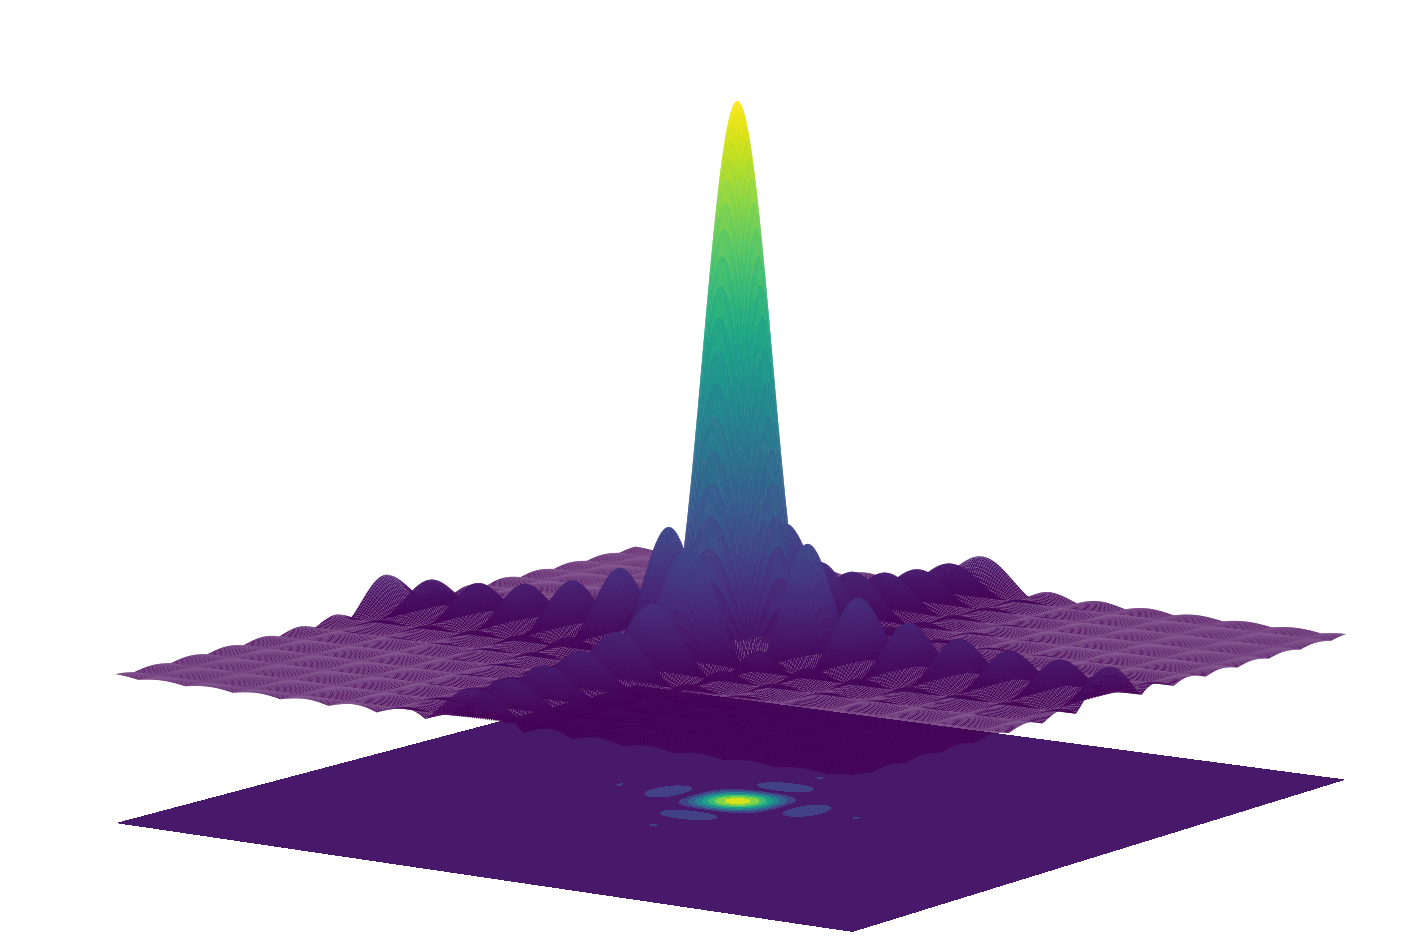
\includegraphics[width = \textwidth]{Ch2_Images/Cubic_aperture.png}
		\caption{cubic aperture}
		\label{cubicAperture}
	\end{subfigure}
	\begin{subfigure}{0.5\linewidth}
		% \centering
		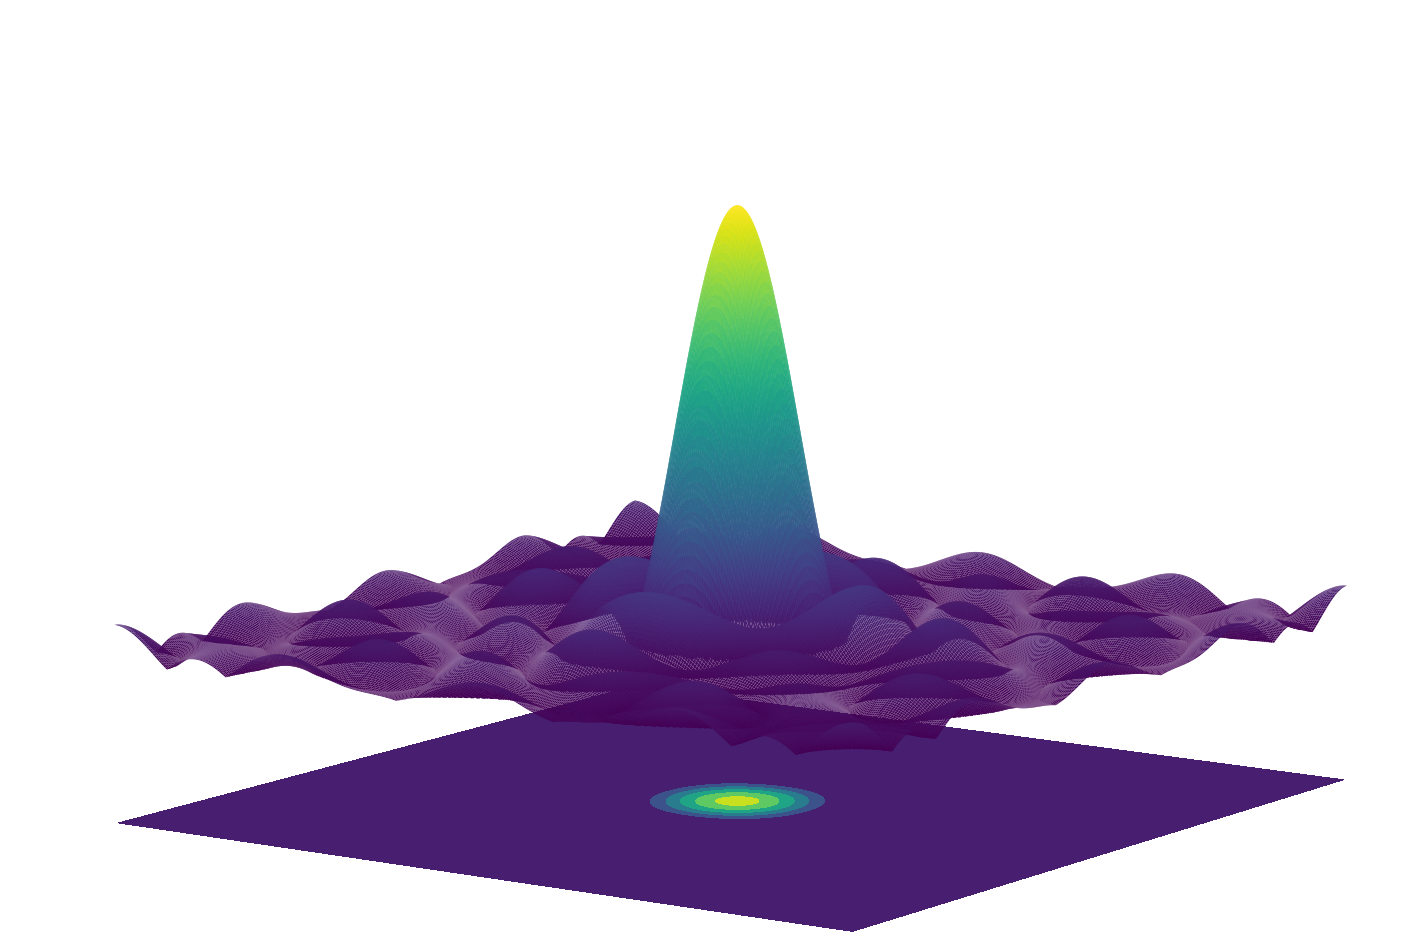
\includegraphics[width = \textwidth]{Ch2_Images/Circular_aperture.png}
		\caption{circular aperture}
		\label{circularAperture}
	\end{subfigure}
\end{figure}
\section{3 images in the same row}
\begin{figure}[htbp!]
\centering
	\begin{subfigure}{0.3\linewidth}
		% \centering
		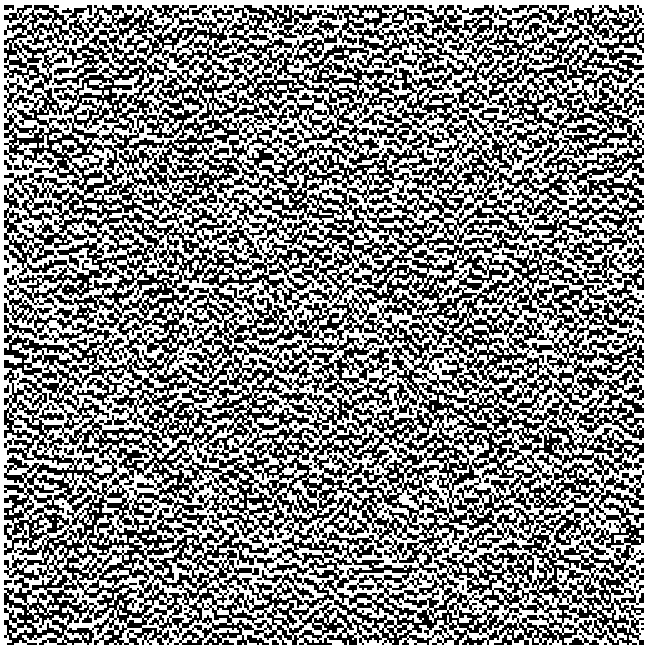
\includegraphics[width = \textwidth]{Ch2_Images/DBS_hologram.png}
		\caption{Place holder 1}
		\label{fig:TargetImage}
	\end{subfigure}
	\begin{subfigure}{0.3\linewidth}
		% \centering
		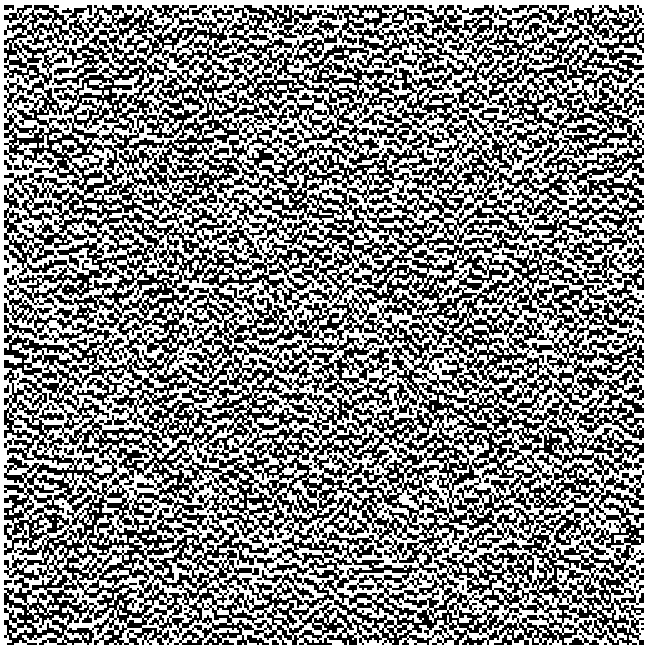
\includegraphics[width = \textwidth]{Ch2_Images/DBS_hologram.png}
		\caption{Place holder 2}
		\label{fig:DBS_Hologram}
	\end{subfigure}
	\begin{subfigure}{0.3\linewidth}
		% \centering
		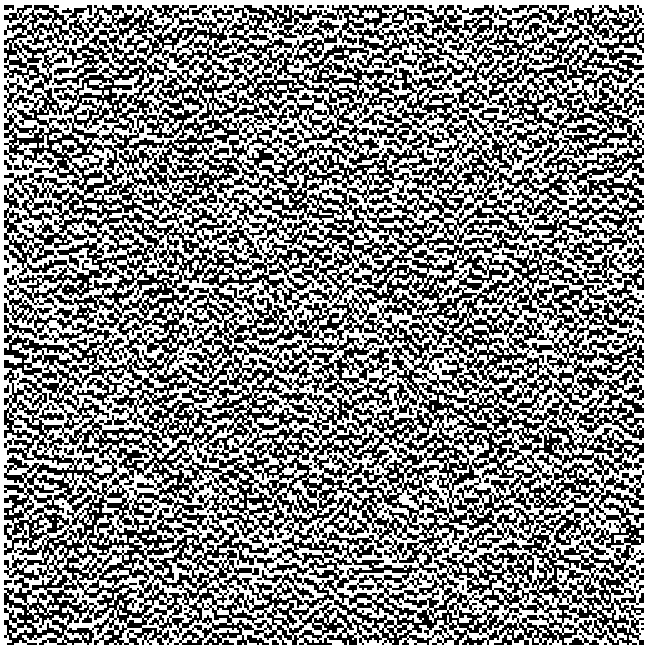
\includegraphics[width = \textwidth]{Ch2_Images/DBS_hologram.png}
		\caption{Place holder 3}
		\label{fig:DBS_replayfield}
	\end{subfigure}
	\caption{Example of position 3 figures}
	\label{fig:DBS_example}
\end{figure}


\section{Algortihm}
\bigskip
%%% Direct Binary Search %%%
\begin{algorithm}[H]
	\SetAlgoNoLine
	\caption{Direct binary search}
	\KwData{\\\textbf{T}: Target replay field\\ $\bm{C_{0,1}}$: Cost function\\
	$\boldsymbol{H_{0,1}}$: Replay field after flipping one pixel}
	\KwIn{\\N: Number of iterations}
	\KwOut{Optimized phase}
	Define the target replay field, \textbf{T}
	Random flip one pixel, and calculate its replay field, $\bm{H_0}$

	\For{\textbf{k $<$ N}}{
	Take the difference between $\bm{T}$ and $\bm{H_0}$, calculate the first cost function $\bm{C_0}$\;
	Random flip one pixel, then calculate its replay field, $\bm{H_1}$\;
	Take the difference between \textbf{T} and $\bm{H_1}$, then find the second cost function $\bm{C_1}$\;
	\uIf{$C_0 < C_1$}{
		Reject the flip and turn it back\;
	}
	\uElseIf{$C_0 > C_1$}{
		Accept the flip and update the old cost function $C_0$ with the new one $C_1$\;
	}
	\textbf{k = k + 1}
}
\end{algorithm}
\bigskip
\cleardoublepage
